\section{Results} 
\label{sec:results}


To test the proposed DSE of security, a mock architecture was defined containing eight components, each with one asset, as seen in Figure \ref{fig:eightcomponents_oneasset} and then placed under three different system constraints: full resources [53,200 LUTs, 15W], restricted LUTs [15,000 LUTs, 15W], and restricted power [53,200 LUTs, 70mW]. The allowed asset risk is 50/50 to allow all possible solutions to be shown. All other values, such as FFs, DSPs, and LUTRAM were defined, but not restricted. Allowable read latency and write latency were defined for each asset in the system architecture. 

\begin{figure}[h]
    \centering
    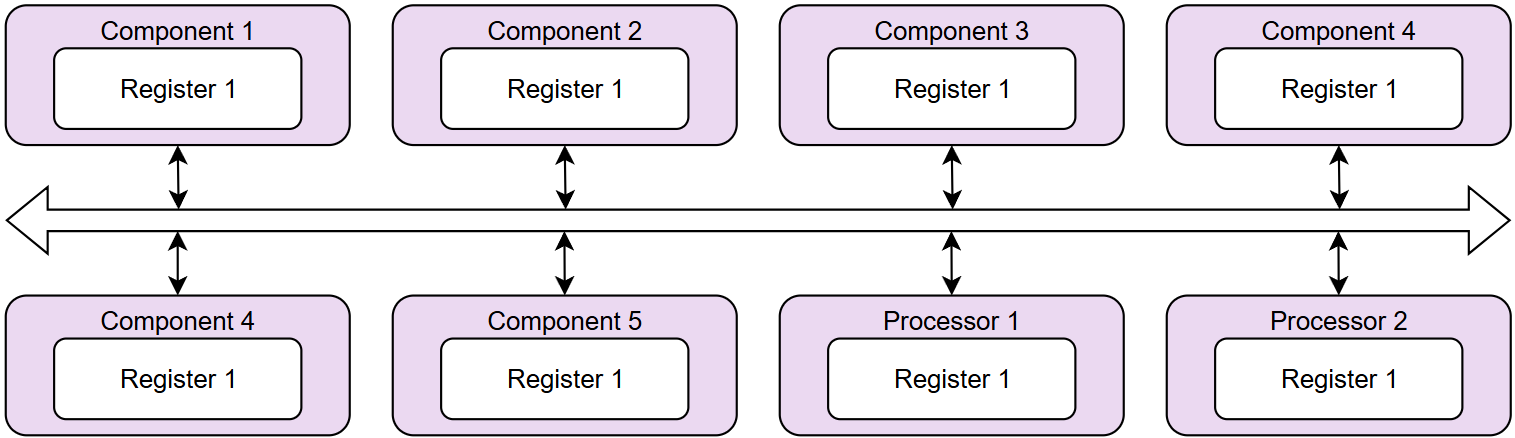
\includegraphics[width=0.45\textwidth]{Images/eightcomponents_oneasset.png}
    \caption{Test Case System-on-Chip, Eight Components, Each With One Asset}
    \label{fig:eightcomponents_oneasset} % caption for the whole figure
\end{figure}

Given the novelty and lack of direct comparisons, as noted in \ref{sec:relatedWorks} this section uses a synthetic benchmark for evaluation. Each DSE returns a set of solutions that fit the user's constraints. For the defined test case, our DSE for Security tool outputs the plots seen in Figure \ref{fig:testCaseResults}. 
Each DSE returns a set of solutions that fit the user's constraints. For the defined test case, the DSE algorithm outputs the plots seen in Figure \ref{fig:testCaseResults}. 


%===================
\begin{figure*}[h]
    \centering
    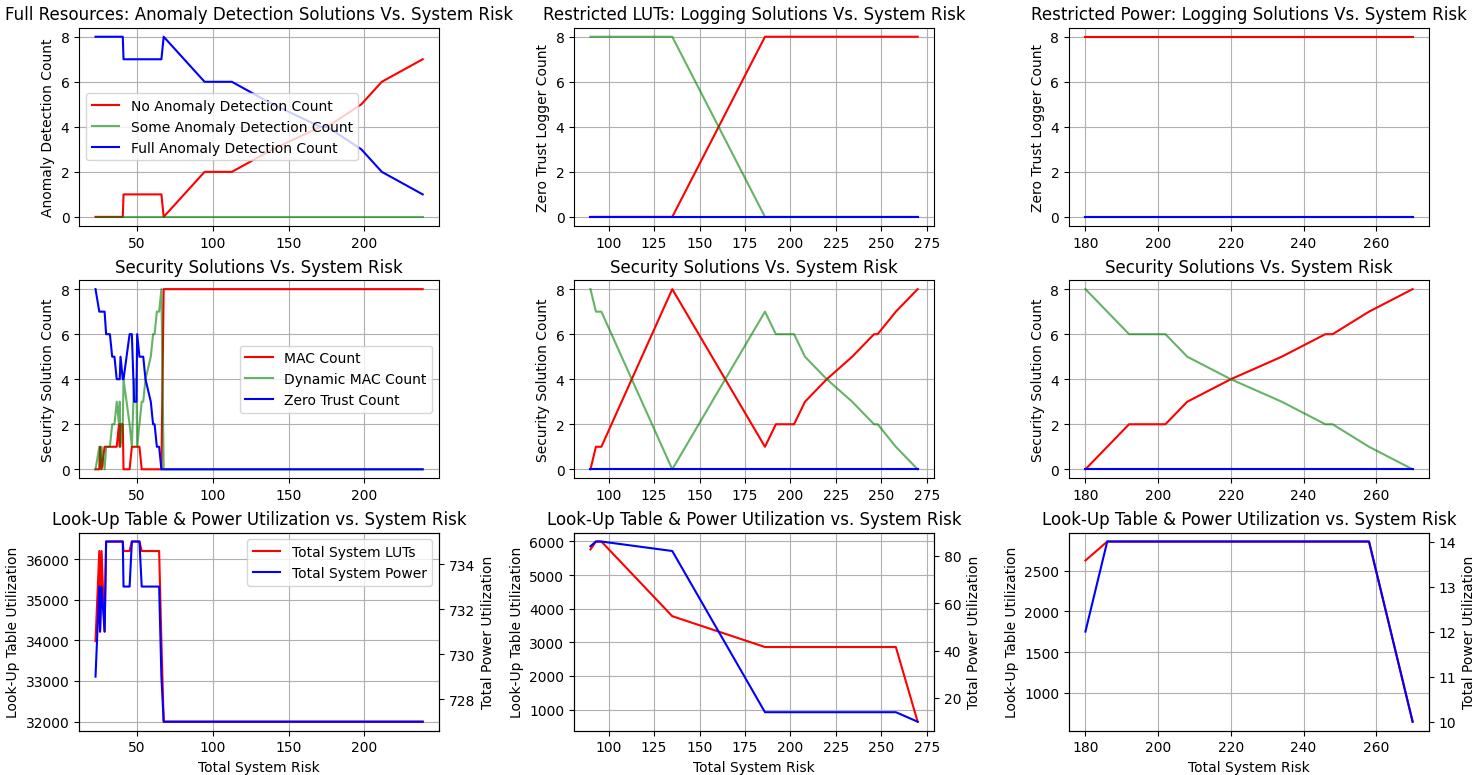
\includegraphics[width=0.86\textwidth]{Images/plotClingo2.png}
    \caption{Selected Anomaly Detection, Security Features, and LUT Utilizatio \& Power Utilization Vs. Total System Risk}
    \label{fig:testCaseResults} % caption for the whole figure
\end{figure*}
%==========================

In Figure \ref{fig:testCaseResults}, each column represents one of the system constraints, with a smaller total system risk being better. For the Full Resources optimization, the solution with the lowest system risk, around 20, the left-most solution, utilized zero-trust anomaly detection, and zero-trust security for every asset, costing 34,000 LUTs, and 729mW of power. Slightly less optimal solutions, between 20 and 60, require more LUTs and power because they simultaneously use two different anomaly detection solutions and three different security solutions. Around the 60 risk mark, there is a notable drop in LUT and power utilization caused by using only MAC security. Here, only the highest risk assets receive zero-trust anomaly detection, and all other assets receive MAC, a lesser protection.

In the Restricted LUTs optimization, the solution with the lowest system risk, around 100, utilized partial anomaly detection and D-MAC security for every asset, costing a total of 5,800 LUTs and 80mW of power. Significantly less optimal solutions, ranging from 175 to 275 system risk, utilized fewer LUTs and power, but did not perform any anomaly detection and utilized MAC security. This solution is only slightly better than a system that has no security at all and was only suggested because the optimizer was allowed to report back asset risks up to 50.

Next, looking at the Restricted power optimization, it can be seen that the solution with the lowest system risk, around 180, utilized no anomaly detection and D-MAC security for every asset, costing a total of 260 LUTs and 12mW of power. There is no drop-off in system risk until around the 260 system risk mark, where MAC becomes the primary security solution. Similar to the least optimal solution in the Restricted LUTs column, the least optimal solution is slightly better than not protecting the system at all. 




%These plots showcase the complexity of making security decisions for a relatively simple system design of eight total assets. The proposed design automation for security tool automatically creates



\subsection{Takeaways from Results}

This work offers designers a comprehensive understanding of the trade-offs between anomaly detection and security solutions, LUT utilization, and power utilization under different optimization constraints. By leveraging this visualized data, designers can more easily make informed decisions to select the appropriate anomaly detection and security solutions that fit their system's needs and constraints. Currently, the tool supports optimizing the system security using three anomaly detection solutions and three security solutions, but it is designed to be extensible, allowing users to incorporate their own features and solutions. %The complexity of the user's design can be as intricate as required, as the tool can handle a wide range of scenarios and configurations.

Finally, given three logging solutions and three security solutions, this leads to nine possible combinations for each asset, and a total of eight assets. A total \(9^8=43,046,721\) possible combinations. The proposed optimizer, under the Full Resources condition, reported back only 43 possible solutions, many of which can be removed by restricting the maximum allowed asset risk. When optimizing on a larger system of 16 assets, the tool reported back only 44 potential solutions in several seconds. This indicates that the proposed method may be scalable. However, larger systems have not been tested.

 


